%&pdflatex
%!TEX TS-program = pdflatex
%!TEX encoding = UTF-8 Unicode
%
% PLANTILLA PARA UN TRABAJO DE FIN DE GRADO
% EN EL GRADO DE MATEMÁTICAS DE LA UNIVERSIDAD DE ZARAGOZA
%
% Mario Pérez Riera
% Área de Análisis Matemático, Universidad de Zaragoza
%
% Última modificación: 1 de agosto de 2021
%
% Escrito para pdfLaTeX
%
%
\documentclass[11pt]{book}

% Paquetes y fuentes
%---------------------------------------------------------------------------
\usepackage{geometry}               % define las dimensiones de la página
\geometry{
 a4paper, % Tamaño del papel
 centering, % Zona útil centrada
 margin = 25mm, % Márgenes en blanco: 25mm
% includehead, % Incluir la cabecera en el área del texto
% includefoot, % Incluir el pie en el área del texto
}

\usepackage[utf8]{inputenc}        % para usar el teclado normalmente
\usepackage[spanish]{babel}        % selecciona idioma
\usepackage[T1]{fontenc}           % gestión de fuentes con acentos
\usepackage{textcomp}

% Si alguno de estos paquetes no los vas a usar, mejor los quitas:
\usepackage{amssymb}               % para cargar las fuentes de la A.M.S.
\usepackage{amsmath}               % para usar letras griegas en negrita
\usepackage{amsthm}                % mejora los entornos tipo-teorema y proof
\usepackage{mathptmx}              % fuente Times
%\usepackage{lmodern}              % fuente Times
\usepackage{tikz}                  % para los dibujos
\usetikzlibrary{babel}              % para evitar conflictos entre TikZ y babel


%\usepackage{longtable}             % permite saltos de páginas en tablas largas

%------ Enlaces en el pdf
\usepackage{url}
\usepackage[linesnumbered,ruled,vlined]{algorithm2e}


\usepackage[pdftex, colorlinks=true, citecolor=cyan, linkcolor=black, 
urlcolor=black]{hyperref}

%------ Cabeceras y pies de página
\usepackage{titleps}

\newpagestyle{miestilo}{
   \sethead[\thepage][][\textsl{\chaptername\ \thechapter. \chaptertitle}]
   {\textsl{Titulo -> Preguntar a Tomás \ - \ Hugo Naudín López}}{}{\thepage}
   %\setfoot[][\textsl{\thesection. \sectiontitle}][]
   %{}{\textsl{\thesection. \sectiontitle}}{}
}

\newpagestyle{primeraparte}{
%-- Cabecera par y cabecera impar
\sethead[\thepage][][\textsl{\chaptertitle}]
{\textsl{Una plantilla para el TFG \ - \ Mario Pérez Riera}}{}{\thepage}
%-- Pie de página par y pie de página impar
%\setfoot[][\textsl{\thesection. \sectiontitle}][]
%{}{\textsl{\thesection. \sectiontitle}}{}
}

%------ \S 4.3, p. 93, de The LaTeX Companion 1a ed. (Figura 4.2) (Juan Luis)
\newcommand{\clearemptydoublepage}{\newpage{\pagestyle{empty}\cleardoublepage}}
\newcommand{\sectionmarkwithoutsections}[1]{\markright{#1}}


\makeindex

\theoremstyle{plain} % Entornos tipo teorema
\newtheorem{teorema}{Teorema}[chapter]
%\newtheorem{lema}[teorema]{Lema} % La misma numeración que 'teorema'
\newtheorem{proposition}{Proposición}
\theoremstyle{definition} % Entornos tipo definición
\newtheorem*{defin}{Definición} % El asterisco hace que no se numere
%\newtheorem{ejemplo}{Ejemplo}

%------ Conjuntos de números
\newcommand\N{\mathbb{N}}
\newcommand\Z{\mathbb{Z}}
\newcommand\R{\mathbb{R}}
\newcommand\C{\mathbb{C}}

%------ Funciones en español
\renewcommand{\spanishoperators}{Re}
%\renewcommand{\spanishoperators}{Re ctg arc\,ctg} % Define \Re, \ctg, \arctg

%-------------
\begin{document}
%-------------
\frontmatter                     % Parte primera del texto
\pagestyle{primeraparte}    % Estilo de cabeceras para la parte primera del texto

%\pagenumbering{roman} % Incluido en \frontmatter

%--- PORTADA DEL TFG
\begin{titlepage}
\begin{center}

\null
\vfill

\Huge{\bfseries Técnicas de aprendizaje autonático aplicadas a la estimación del Valor a Riesgo y otras medidas de riesgo financiero}

\vfill

\noindent
\begin{figure}[h]
\centering

\includegraphics[width=100mm]{ciencias.png}\\%

\includegraphics[width=100mm]{logoUZ.png}
\end{figure}

\vfill

\Huge{\bfseries Hugo Naudín López}\\%
\Huge{Trabajo de fin de grado de Matemáticas}\\%
\Huge{Universidad de Zaragoza}\\%

\vfill
\huge{Junio de 2025}
\end{center}
\end{titlepage}
%--- FIN DE LA PORTADA

\clearemptydoublepage

%\setcounter{page}{7} % Por si queremos imponer un número de página

%--- RESUMEN
\chapter{Resumen}

Este documento es una plantilla en {\LaTeX} diseñada para cumplir con las 
\emph{directrices propias} para la elaboración del trabajo de fin de grado de 
Matemáticas en la Facultad de Ciencias de la Universidad de Zaragoza. Estas 
directrices, que se pueden ver en~\cite{FC}, indican lo siguiente sobre la 
memoria (artículo $4$):

\begin{enumerate}
\item La memoria del TFG podrá ser redactada en español o en inglés. Si la 
memoria está escrita en español (respectivamente en inglés) deberá acompañarse de 
un resumen en inglés (respectivamente en español). La extensión de dicho resumen 
será de dos o tres páginas.

\item La memoria se editará, preferiblemente, utilizando el sistema de 
composición de documentos {\LaTeX}. A tal efecto, en la página web de la Facultad 
de Ciencias se dispondrá de una plantilla~{\LaTeX}.

\item Con el fin de facilitar su validación administrativa, todas las memorias de 
TFG de la Facultad de Ciencias tendrán un tamaño de letra diferenciado mínimo 
de~$11$ puntos, con un interlineado a espacio $1.15$ y márgenes de al menos 
$2.5$~cm, en papel tamaño DIN A4. El índice y el resumen deberán ir justo antes 
del inicio de la memoria y esta, en ningún caso, podrá superar las $25$ páginas, 
excluidos los anexos.

\item El director de un TFG deberá comprobar que la memoria presentada cumple con 
las normas de edición establecidas, antes de dar el visto bueno a su depósito.
\end{enumerate}

Esta plantilla se ofrece por si resulta útil, pero 
debe quedar claro que no es obligatorio usarla: el trabajo se puede escibir prescindiendo de esta plantilla, siempre que se respeten las directrices anteriores.

La plantilla está diseñada para un trabajo compuesto por uno o más capítulos y una 
bibliografía única, es decir, no una por cada capítulo. Detallando un poco más, 
la estructura es la siguiente y por este orden:
\begin{itemize}
\item Una portada.
\item Un resumen.
\item Después, un índice general en el que figuran el resumen, los capítulos de 
los que consta el trabajo y la bibliografía. 
Cada capítulo puede contener secciones, que también aparecen en el índice.
\item La parte principal, formada por cada uno de los capítulos que componen el 
trabajo.
\item Y, por último, la bibliografía.
\end{itemize}

La plantilla está escrita para componerse en \texttt{pdflatex} y la forman varios 
archivos que deben estar en la misma carpeta:
\begin{itemize}
\item Un documento principal, que contiene las órdenes iniciales y el código \LaTeX del texto.
\item Los archivos de imágenes que se vayan a incluir en el trabajo.
\end{itemize}

En el primer capítulo de este modelo se dan más detalles sobre esta plantilla.

Obsérvese que en este ejemplo el resumen no sigue las directrices 
establecidas para los trabajos de fin de grado, según las cuales debe estar 
escrito en inglés si el trabajo está en castellano.

El último capítulo de este documento se ha puesto solo como relleno, como ejemplo 
de texto matemático, y no corresponde a un verdadero trabajo de fin de grado.

%--- FIN DEL RESUMEN

\clearemptydoublepage

\tableofcontents

\clearemptydoublepage

%-------------
\mainmatter                      % Parte principal del texto
\pagestyle{miestilo}    % Estilo de cabeceras para la parte principal del texto

%--- CAPÍTULO 1 DEL TFG
\chapter{Introducción: el riesgo en las coporaciones}
A la hora de invertir, el interés de las corporaciones financieras es maximizar 
el beneficio y minimizar las pérdidas. Para ello, las compañías utilizan 
herramientas entre las que se encuentra la gestión del riesgo. El riesgo 
es la incertidumbre sobre la evolución de un activo, e indica la posibilidad 
de que una inversión ofrezca un rendimiento distinto del esperado, por lo 
que la gestión y el control de él puede ayudar a minimizar las pérdidas y 
optimizar las ganancias.\\

Durante la decada de los 80, la Comisión de Bolsa y Valores de los Estados 
Unidos (SEC) comenzó a divulgar cómo las empresas estaban expuestas a la 
volatilidad de los mercados financieros, introduciendo y dando gran 
importancia al concepto de riesgo en el sistema, debido a los acontecimientos 
vividos en aquel entonces (Lunes Negro en 1987 y la Crisis de Ahorros y 
Prestamos). Más adelante, a partir de la crisis financiera del año 2008 y el 
acuerdo de Basilea III, las políticas del riesgo que podían correr los bancos 
a la hora de conceder créditos y realizar inversiones se endurecieron, lo que 
hizo que los modelos de predicción y gestión de riesgo se optimizaran y 
mejoraran de manera considerable.\\

Por otra parte, el uso de la inteligencia artificial (IA) y los algoritmos basados 
en el aprendizaje automático han incrementado en los últimos años, llegando 
a introducirse también en el campo financiero y en la implementación de 
modelos alternativos a la hora de gestionar el riesgo. \\

Para medir el riesgo, existen una gran cantidad de métodos y medidas 
utilizadas globalmente para ayudar a las entidades financieras a tomar 
decisiones. Entre ellas, destaca el Valor a Riesgo 

\section{Valor a Riesgo (VaR)}
Se define el Valor a Riesgo (VaR) como la cuantía máxima de dinero que 
puede perderse en un período para un nivel específico de confianza. Es decir, 
si definimos $G_t$ como los beneficios que obtenemos de una inversión 
en un tiempo $t$ (pueden ser negativos), entonces:
\begin{align*}
     \mathbb{P}\{G_t \leq VaR_{\alpha, t}\} = 1-\alpha
\end{align*}
con $\alpha$ un nivel de confianza específico.
Por otro lado, tomamos unas variables aleatorias que simbolizan las 
ganancias y pérdidas de una inversión en un tiempo $t$, $G_t$, las cuales 
siguen una distribución $F$. Entonces, podemos definir el VaR como:
\begin{align*}
    VaR_{\alpha, t} = inf\{x\in \mathbb{R}:F(x)\geq 1-\alpha\}
\end{align*}
Es decir, dados unos datos empiricos de ganancias (las pérdidas son negativas), 
el VaR representa el cuantil $\alpha$ de la distribución empírica, y por tanto:
\begin{align*}
    VaR_{\alpha, t} = F^{-1}(1-\alpha)
\end{align*}

\subsection{Ventajas y desventajas del VaR}
La medida VaR tiene una gran utilidad a la hora de limitar el riesgo y 
controlar las potenciales pérdidas (o retornos inferiores a lo esperado) 
de una inversión, pero hay otros aspectos en los que esta medida no es 
completa.\\

Por una parte, es una medida muy simple e intuitiva. Su significado y lo que 
represnta son fácilmente comprendible, lo que hace que su utilización este 
muy extendida. Además, la comparabilidad de dos distribuciones se puede 
realizar fácilmente mediante esta medida, lo que puede resultar útil para 
evaluar diferentes carteras o estrategias de inversión en términos de su riesgo 
potencial. Por ejemplo, al comparar dos activos, el VaR permite identificar 
cuál de ellos tiene una mayor probabilidad de incurrir en pérdidas superiores 
a un cierto umbral en un horizonte de tiempo definido. Esto facilita la toma 
de decisiones por parte de gestores de riesgo e inversionistas. Finalmente, 
hay en ocasiones en las que interesa la estabilidad de las medidas de riesgo. 
A la hora de hallar el VaR de una distribución, cualquier cuantil inferior al 
$1-\alpha$ puede tener cualquier valor, pero el VaR no variará, ya que es 
independiente de estos valores, siempre y cuando sean menores.\\

Sin embargo, que el VaR no varíe aunque los cuantiles menores sí, puede ser 
negativo desde otro punto de vista. Esto significaría que una mínima variación 
del nivel de confianza significaría una gran variación del VaR. Por tanto, esta 
medida estaría ocultando un riesgo mayor al que parece en un principio. \\

Esta desventaja hace del VaR una medida que, a pesar de su gran utilidad, 
presenta una notable incompletitud. Por ello, existen otras medidas que 
complementan a esta primera, ofreciendo una extensión a la información del 
VaR, sobre todo, dando información del cuantil inferior. Entre estas 
variables se encuentra el Expected Shortfall (ES) o Valor a Riesgo
Condicional (CVaR). 

\section{Expected Shorfall (ES) o Valor a Riesgo Condicional (CVaR)}
El Expected Shorfall (ES) o Valor a Riesgo Condicional (CVar) son dos términos
relacionados con el mismo concepto. Para no sobrecargar, se referirá a este 
concepto como ES de aqui en adelante. El ES es una medida complementaria 
al VaR que se define como la perdida esperada en una inversión sabiendo 
que la perdida es mayor que el valor del VaR. Por tanto,dado $G_t$ un 
beneficio de una inversión en el tiempo $t$, formalmente definimos:
\begin{align*}
    ES_{\alpha, t} = \mathbb{E}(G_t|G_t \leq VaR_{\alpha, t})
\end{align*}
El ES siempre será una beneficio menor al representado por el VaR, ya que 
el ES toma en cuenta los beneficios menores a él y, por lo, tanto refleja una 
evaluación más conservadora del riesgo. Si el VaR se considera como el 
valor máximo de pérdida en un nivel de confianza $\alpha$, el ES estima 
el valor promedio de las pérdidas cuando las pérdidas ya superan ese valor. 
Por lo tanto, el ES proporciona una medida más completa del riesgo 
asociado a eventos extremos.

\subsection{Ventajas y desventajas del ES}
La medida ES, al contrario del VaR, es una medida continua respecto a $\alpha$, 
es decir, cambios pequeños en el nivel de confianza no suponen cambios 
grandes en el CVaR, que describe como es la perdida esperada extrema, en 
caso de haberla. Si tomamos una sucesión de inversiones $(X_i)_{i=1}^n$ y un 
valor asociado a cada una de ellas $(w_i)_{i=1}^n$, el cual representa la 
proporción que representa esa inversión en el total de nuestra cartera 
($\sum_{i=1}^n w_i = 1$), entonces la medida ES en un tiempo $t$ con una 
confianza $\alpha$ es convexa respecto a la  combinación de estas variables:
\begin{align*}
   ES_{\alpha, t}(w_1X_1+\dots w_nX_n) \leq w_1ES_{\alpha, t}(X_1)+\dots w_nES_{\alpha, t}(X_n)
\end{align*}
lo cual es coherente con la idea de la diversificación de activos para la 
reducción del riesgo, ya que el ES de la cartera nunca excede el promedio 
ponderado de los ES individuales\\

Por otro lado, esta medida es muy sensible a los errores de estimación. 
Normalmente, no existen muchos datos de los cuantiles bajos, por lo que es 
necesario realizar un modelo para obtener más datos. Existen casos en los 
que estos modelos son erráticos y los datos en las colas pueden desviarse de 
la realidad.\\

Por tanto, la utilización y correción de esta medida depende en gran parte 
de la corrección y confianza que tengamos en los datos. Sin embargo, 
la combinación de esta medida con el VaR ofrece una visión muy 
completa del riesgo en la inversión.

\section{Interés de las medidas de riesgo}
Las medidas de riesgo, como el Valor en Riesgo (VaR) y Experted Shorfall (ES), 
son herramientas fundamentales en la gestión de riesgos, ya que permiten 
cuantificar y gestionar la incertidumbre asociada a las pérdidas potenciales 
en diferentes contextos. Su utilidad varía dependiendo de si se aplican a 
carteras de valores o al ámbito corporativo.
\subsection{VaR y ES orientado a carteras de valores}
En el ámbito de la gestión de carteras de inversión, el VaR y el ES son 
cruciales para entender y controlar la exposición al riesgo.\\

En el caso del VaR, estima la pérdida máxima de una cartera de valores 
en un horizonte temporal específico y con un nivel de confianza dado. 
Permite a los gestores de carteras evaluar riesgos acumulativos, 
identificando el impacto potencial de eventos de mercado extremos sobre 
la cartera, tomar decisiones informadas, comparando diferentes estrategias 
de inversión en función de su perfil de riesgo y cumplir requisitos 
regulatorios (normativas de Basilea).\\

El ES complementa al VaR al estimar la pérdida promedio en los casos en 
que esta exceda el VaR. Es especialmente útil porque ofrece una visión más 
completa y optimiza carteras.\\

Las dos medidas juntas son esenciales para medir y gestionar el riesgo de 
mercado, mejorar la asignación de activos y proteger a los inversores frente 
a pérdidas inesperadas.

\subsection{VaR y ES orientado a inversiones inmobiliarias}
La utilización de estas medidas de riesgo en las inversiones inmobiliarias 
se enfoca en la predicción del precio de los alquileres de los inmubles. 
Dado el precio de una vivienda, el VaR y el ES estiman escenarios negativos 
de precios a los que puede ser alquilado, permitiendo estimar 
si la inversión es suficientemente rentable.\\

Al mismo tiempo, el VaR y el ES se pueden utilizar para calcular una 
cota inferior del valor intrínseco de una vivienda dadas unas características
específicas, como la ubicación, el tamaño y las condiciones del mercado.
Esto permite a los inversores evaluar si el precio de compra de una propiedad
es razonable en relación con su valor potencial de alquiler y su riesgo asociado.\\


\subsection{VaR y ES orientadas a corporaciones}
En el contexto corporativo, estas métricas ayudan a evaluar el riesgo 
financiero y operativo que enfrentan las empresas en sus actividades.\\

El VaR se utiliza para medir riesgos asociados a las fluctuaciones en tipos de 
cambio, tasas de interés o precios de materias primas y a la toma de 
decisiones estratégicas.\\

Por su parte el ES proporciona una perspectiva más amplia, considerando 
las pérdidas extremas que pueden no ser capturadas por el VaR. Ofrece un 
análisis más detallado de los escenarios de mayor impacto financiero y 
permite a las empresas diseñar planes de mitigación y estrategias para 
afrontar eventos inesperados.\\

En el ámbito corporativo, estas medidas de riesgo facilitan la identificación 
de vulnerabilidades clave, la planificación financiera y la protección de los 
recursos de la empresa frente a incertidumbres del entorno operativo y del 
mercado.

\subsection{VaR y ES orientado a predicciones de impago en créditos}
Estas variables económicas también se emplean en la predicción de impago 
de créditos, lo que ayuda a los bancos y entidades de prestamos en sus 
decisiones.
El VaR se utiliza para estimar la cantidad que con una probabilidad dada 
el cliente impagará, considerando factores como el historial crediticio, la 
situación financiera, las condiciones del mercado y determinadas 
carácteristicas del cliente. \\

Por otra parte, el ES, al igual que en el caso de las carteras de valores, se 
utiliza para evaluar la pérdida promedio en los casos en que el cliente no 
pague, lo que da más información a la entidad acerca de la rentabilidad de 
dar el crédito.\\

Estas medidas permiten a las entidades evaluar el riesgo asociado a la 
concesión de créditos y ajustar sus políticas de préstamo en consecuencia.\\


\clearemptydoublepage
\chapter{Modelos de riesgo}
%--- CAPÍTULO 2 DEL TFG
Con el objetivo de aproximar las medidas de riesgo anteriormente descritas, 
a lo largo de la historia se han ido desarrollando diferentes modelos, que 
emplean técnicas distintas, que ayudan a predecir el riesgo dadas distintas 
situaciones.
\section{Modelos tradicionales}
Los métodos tradicionales están fundamentados en la econometría y en 
métodos estadísticos. Sin embargo, estos enfoques pueden presentar 
limitaciones cuando se enfrentan a condiciones de mercado altamente 
volátiles o a eventos inesperados. Además, algunos se basan en suposiciones 
no siempre ciertas (distribuciones normales, independencia de errores, etc.). 
Sin embargo, existen otras técnicas que tienen una mayor robustez. 
\subsection{Regresión cuantil}
La regresión cuantil es un método estadístico que permite estimar la 
relación entre variables explicativas con los cuantiles de la distribución 
de la variable dependiente. A diferencia de la regresión lineal usual, 
que se centra en la media condicional, la regresión cuantil proporciona una 
visión más completa de la relación entre variables al considerar los cuantiles 
de la distribución, de donde podemos obtener una información mayor.\\

Para introducir la regresión cuantil, veamos primero las bases de la regresión 
lineal. Tomamos unas variables explicativas $\mathbf{X_i} = \{X_{i1}, X_{i2}, \dots, X_{ik}\}$ 
y una variable dependiente $Y_i$. La regresión lineal se basa en la suposición 
de que existe una relación entre las variables explicativas y la variable 
dependiente  y se puede expresar de la siguiente manera:
\begin{align*}
    Y_i = \beta_0 + \beta_1X_{i1}+\beta_2X_{i2}+ \cdots + \beta_k X_{ik}+\epsilon_i
\end{align*}
con $\epsilon$ una variablede ruido que sigue una distribucion $N(0, \sigma)$
dado un $\sigma$ cualquiera. Es decir, existe un vector 
$\mathbf{\beta} = (\beta_0, \beta_1, \dots, \beta_k)$ tal que:
\begin{align*}
    Y_i = \mathbf{\beta} \cdot \mathbf{X_i} + \epsilon_i
\end{align*}

Los coeficientes $\beta_i$ representan la relación entre las variables y se 
denominan coeficientes de regresión. El objetivo de la regresión lineal es 
obtener unos coeficientes $\hat{\beta}_{ik}$:
\begin{align*}
   \hat{Y}_i = \hat{\beta}_0 + \hat{\beta}_1X_{i1}+\hat{\beta}_2X_{i2}+\cdots + \hat{\beta}_k X_{ik}
\end{align*}
tal que la suma de los errores al cuadrado sea mínima. Es decir, queremos obtener
$\hat{\beta} = (\hat{\beta}_0, \hat{\beta}_1, \dots, \hat{\beta}_k)$ tal que: 
\begin{align*}
    \mathbf{\hat{\beta}} = argmin_{\beta}\sum_{i=1}^n(Y_i-\hat{Y}_i)^2
\end{align*}

La regresión cuantil, por otro lado, intenta modelar el cuantil $\alpha$ de la 
variable dependiente $Y_i$ dado un conjunto de variables explicativas 
$\mathbf{X_i}$, en vez de centrarse en la media. La forma general del modelo es:
\begin{align*}
    c_{\alpha}(Y_i|\mathbf{X}_i) = \dot{\beta}_0(\alpha)+ \dot{\beta}_1(\alpha)X_{i1}+ \dot{\beta}_2(\alpha)X_{i2}+\cdots +  \dot{\beta}_k(\alpha)X_{ik}
\end{align*}
donde $c_{\alpha}(Y_i|\mathbf{X}_i)$ es la estimación del cuantil $\alpha$ de la 
variable dependiente $Y_i$ dado el vector de variables explicativas 
$\mathbf{X}_i$.\\

Paralelamente a lo anterior, para hallar los coeficientes de regresión 
$\dot{\beta} = (\dot{\beta}_0(\alpha), \dot{\beta}_1(\alpha), \dots, \dot{\beta}_k(\alpha))$
debemos hallar los valores que minimicen una función de pérdida cuantílica. 
En este caso, esta función va ser diferente a la anterior:
\begin{align*}
    \mathbf{\dot{\beta}}(\alpha) = argmin_{\beta}\sum_{i=1}^n\rho_{\alpha}(Y_i-c_{\alpha}(Y_i|\mathbf{X}_i))
\end{align*}
con $\rho_{\alpha}(r) = r \cdot (\alpha - I(r<0))$ la función de pérdida cuantílica.
\begin{proposition}
      Sea $X$ una variable aleatoria continua con función de distribución $F$ y 
      cuantil $\alpha$, y dada la función de pérdida cuantílica:
      \begin{align*}
            p_{\alpha}(r) = r(\alpha - I(r<0))
      \end{align*}
      Tomando una variable $\theta$ y la función:
      \begin{align*}
            E_x(p_{\alpha}(X-\theta)) = \int p_{\alpha}(x-\theta)f_x(x)dx
      \end{align*}
      entonces, el valor de $\theta$ que minimiza la función es el cuantil $\alpha$ 
      de la variable aleatoria $X$.
\end{proposition}

\begin{proof}
   Nuestro objetivo es ver que:
   \begin{align*}
      c_{\alpha}(X) &= \inf\{x\in \mathbb{R}:F(x)\geq \alpha\} = argmin_{\theta}\left\{E_x(p_{\alpha}(X-\theta))\right\}\\
   \end{align*}
   Para demostrarlo, vamos a ver que el valor de $\theta$ que minimiza la 
   función $E_x(p_{\alpha}(X-\theta))$ es el cuantil $\alpha$ de la variable 
   aleatoria $X$:
   \begin{align*}
       E_X(p_{\alpha}(X-\theta)) &= \int p_{\alpha}(x-\theta)f_x(x)dx\\
       &= \int _{-\infty}^{\infty}(x-\theta)(\alpha - I(x-\theta<0))f_x(x)dx\\
       &= \int_{-\infty}^{\theta}(x-\theta)(\alpha -1)f_x(x)dx+\int_{\theta}^{\infty}(x-\theta)\alpha f_x(x)dx\\
       &= (\alpha -1)\int_{-\infty}^{\theta}(x-\theta)f_x(x)dx+\alpha \int_{\theta}^{\infty}(x-\theta) f_x(x)dx\\
       &= (\alpha -1)\int_{-\infty}^{\theta}xf_x(x)dx-(\alpha -1)\theta \int_{-\infty}^{\theta}f_x(x)dx+\alpha \int_{\theta}^{\infty}x f_x(x)dx-\alpha \theta \int_{\theta}^{\infty} f_x(x)dx\\
   \end{align*}
   Como queremos minimizar esta función con respecto a theta, queremos 
   que su derivada sea nula, por lo que derivando con respecto a $\theta$:
   \begin{align*}
       0 &= -(\alpha -1) \int_{-\infty}^{\theta}f_x(x)dx-\alpha  \int_{\theta}^{\infty} f_x(x)dx\\
       0 &= -(\alpha -1) (F(\theta)-F(-\infty))- \alpha (F(\infty)-F(\theta))\\
       0 &= -(\alpha -1) F(\theta)-\alpha (1-F(\theta))\\
       0 &= -\alpha F(\theta)+F(\theta) -\alpha+\alpha F(\theta) \\
       0 &= F(\theta)-\alpha \implies \theta = F^{-1}(\alpha )
   \end{align*}
   Por tanto, el valor de $\theta$ que minimiza la función es el cuantil $\alpha$ de la variable aleatoria $X$.
\end{proof}
Un vez estimamos los coeficientes, podremos hacer una predicción de los 
cuantiles de la variable dependiente $Y_i$ dado un conjunto de variables 
explicativas $\mathbf{X_i}$.\\

La utilidad de la regresión cuantil reside, entre otras, en la facilidad para 
el cálculo del VaR, ya que permite estimar beneficios extremadamente bajos 
(incluso negativos) y relacionarlos con otros factores como las tasas de interés,
los precios de las materias primas o las condiciones del mercado, todo ello 
sin depender de la media ni de supuestos de normalidad.


\subsection{Regresión expectil}
Además de los cuantiles, existe una medida estadística de gran utilidad 
para la estimación del riesgo. El expectil $\tau$ ($e_\tau$) de una variable 
aleatoria $X$ es aquel valor que minimiza la función $\phi(X-e_\tau)$, donde:
\begin{align*}
   \phi(r) = 
   \begin{cases}
         \tau \cdot  r^2 & \text{si } r \ge 0 \\
         (1 - \tau)r^2 & \text{si } r < 0
   \end{cases}
\end{align*}

Los expectiles se pueden utilizar como una aproximación de los cuantiles, 
aunque no son exactamente lo mismo. Mientras que los cuantiles dividen la
distribución en partes iguales, los expectiles ponderan las pérdidas de manera
diferente, dando más peso a pérdidas extremas. Por tanto, la aproximación 
no es la manera correcta de usarlos. \\

La regresión expectil es un método estadistico útil para estimar variables 
relacionadas con la cola de una distribución como, por ejemplo, 
el Expected Shortfall (ES). 
Mientras que la regresión cuantil minimiza una función de pérdida absoluta 
asimétrica, la regresión expectil minimiza una función de pérdida cuadrática 
asimétrica.\\

Dadas unas variables explicativas $\mathbf{X_i} = \{X_{i1}, X_{i2}, \dots, X_{ik}\}$ y 
una variable dependiente $Y_i$, la regresión expectil se define como:
\begin{align*}
    e_\tau(Y_i|\mathbf{X_i})= \bar{\beta}_{0}(\tau)+ \bar{\beta}_{1}(\tau)X_{i1}+ \bar{\beta}_{2}(\tau)X_{i2}+\cdots +  \bar{\beta}_{k}(\tau)X_{ik} = \bar{\beta}(\tau)  \mathbf{X_i}
\end{align*}
y cumple lo siguiente:
\begin{align*}
    \bar{\beta}(\tau) = argmin_{\beta}\sum_{i=1}^n\phi_{\tau}(Y_i-e_{\tau}(Y_i|\mathbf{X}_i))
\end{align*}

\begin{proposition}
   Dado $ES_\alpha$ el Expected Shortfall de una variable aleatoria $X$ de grado $\alpha$, 
   podemos expresarlo en funcion de $e_\tau$ el expectil ($ES_\tau = g(e_\tau)$) con 
   $e_\tau$ cumpliendo $P(X \leq e_\tau) = \alpha$. 
\end{proposition}
\begin{proof}
   En primer lugar definimos ambos conceptos.Vamos a tomar X la variable
   aleatoria que representa unas ganancias. El Expected Shortfall (ES)
   es la esperanza de los beneficios que no superan el VaR, es decir:
   \begin{align*}
       ES_\alpha = \mathbb{E}(X|X\leq VaR_\alpha) = \mathbb{E}(X|X\leq F^{-1}(\alpha))
   \end{align*}
   Por otro lado, el expectil es el valor que minimiza la función:
   \begin{align*}
       \begin{cases}
           \tau(X - e_\tau)^2 & \text{si } X \ge e_\tau \\
           (1 - \tau)(X - e_\tau)^2 & \text{si } X < e_\tau
       \end{cases}
   \end{align*}
   Podemos definir también esta función como:
   \begin{align*}
       \phi_{\tau}(X - e_\tau) &= \tau(X - e_\tau)^2 I(X \ge e_\tau) + (1 - \tau)(X - e_\tau)^2 I(X < e_\tau) \\
        &= (\tau I(X \ge e_\tau) + (1 - \tau)I(X < e_\tau))(X - e_\tau)^2 \\
   \end{align*}
   Vamos a desarrollar y obtener propiedades del expectil. Para ello, 
   vamos a tomar $\theta$ y a ver cual es  el valor de $\theta$ que minimiza 
   la esperanza de la función.
   \begin{align*}
      g_{\tau, \theta}(X) = (\tau I(X \ge \theta) + (1 - \tau)I(X < \theta))(X - \theta)^2 
   \end{align*}
   Vemos su esperanza:
   \begin{align*}
      E_{X}(g_{\tau, \theta}(X)) &= E_{X}((\tau I(X \ge \theta) + (1 - \tau)I(X < \theta))(X - \theta)^2) = \\
      &= \int_{-\infty}^{\infty}(\tau I(x \ge \theta) + (1 - \tau)I(x < \theta))(x - \theta)^2 f_X(x)dx = \\
      &= \int_{-\infty}^{\theta}((1 - \tau)(x - \theta)^2 f_X(x)dx + \int_{\theta}^{\infty}(\tau (x - \theta)^2 f_X(x)dx = \\
      &= (1 - \tau)\int_{-\infty}^{\theta}(x - \theta)^2 f_X(x)dx + \tau \int_{\theta}^{\infty}(x - \theta)^2 f_X(x)dx
   \end{align*}
   Derivamos con respecto a theta
   \begin{align*}
      \frac{d}{d\theta}E_{X}(g_{\tau, \theta}(X)) &= (1 - \tau)\int_{-\infty}^{\theta}2(x - \theta)f_X(x)dx + (1 - \tau)(\theta - \theta)^2 f_X(\theta) + \\
      &\quad + \tau\int_{\theta}^{\infty}2(x - \theta)f_X(x)dx + \tau(\theta - \theta)^2 f_X(\theta) = \\
      &= (1 - \tau)\int_{-\infty}^{\theta}2(x - \theta)f_X(x)dx + 2\tau\int_{\theta}^{\infty}(x - \theta)f_X(x)dx = \\
      &= 2((1-\tau)E_{X}((X-\theta)\cdot 1_{X\leq \theta}) + \tau E_{X}((X-\theta)\cdot 1_{X >\theta})) = 0
   \end{align*} 
   Por tanto, simplificando, tenemos que:
   \begin{align*}
      E_{X}((X-\theta)\cdot 1_{X\geq \theta}) = -\frac{\tau}{1-\tau}E_{X}((X-\theta)\cdot 1_{X<\theta})
   \end{align*}
   y sustituyendo $\theta$ por $e_\tau$, tenemos que:
   \begin{align*}
      E_{X}((X-e_\tau)\cdot 1_{X\geq e_\tau}) = -\frac{1-\tau}{\tau}E_{X}((X-e_\tau)\cdot 1_{X<e_\tau})
   \end{align*}
   denotamos $A = E_{X}((X-e_\tau)\cdot 1_{X\geq e_\tau})$ y $B = E_{X}((X-e_\tau)\cdot 1_{X<e_\tau})$, por lo que:
   \begin{align*}
      A = -\frac{1-\tau}{\tau}B
   \end{align*}
   Sabiendo que $\alpha = P(X \leq e_\tau)$, por lo que:
   \begin{align*}
      E_{X}((X-e_\tau)\cdot 1_{X \leq e_\tau}) &= \int_{-\infty}^{e_\tau}(x-e_\tau)f_X(x)dx = \int_{-\infty}^{e_\tau}xf_X(x)dx - e_\tau \int_{-\infty}^{e_\tau}f_X(x)dx = \\
      &= \frac{\alpha}{\alpha}\int_{-\infty}^{e_\tau}xf_X(x)dx - e_\tau \alpha = \alpha (ES_\alpha - e_\tau)
   \end{align*}
   Por tanto, despejando $ES_\alpha$:
   \begin{align*}
      ES_\alpha &= \frac{1}{\alpha}E_{X}((X-e_\tau)\cdot 1_{X \leq e_\tau}) + e_\tau
   \end{align*}
   Queremos una expresión más sencilla. Sumamos A y B, calculados anteriormente:
   \begin{align*}
      A + B &= E_{X}((X-e_\tau)\cdot 1_{X\geq e_\tau}) + E_{X}((X-e_\tau)\cdot 1_{X<e_\tau}) = \\
      &= E_{X}(X-e_\tau) = E_{X}(X) - e_\tau
   \end{align*}
   Al mismo tiempo, 
   \begin{align*}
      A+B = -\frac{1-\tau}{\tau}B + B = \left(1 - \frac{1-\tau}{\tau}\right)B = \frac{2\tau-1}{\tau}B 
   \end{align*}
   Por tanto, sustituyendo en la expresión anterior:
   \begin{align*}
      ES_\alpha &= \frac{1}{\alpha}B + e_\tau = \frac{1}{\alpha}E_{X}((X-e_\tau)\cdot 1_{X \leq e_\tau}) + e_\tau = \\
      &= \frac{\tau}{\alpha \cdot (2\tau-1)} (E_X(X)-e_\tau)+e_\tau \\
   \end{align*}

\end{proof}
Por tanto, utilizaremos la regresión expectil para estimar que valor de $\tau$
es el más adecuado para que el expectil $e_\tau$ coincida con el VaR 
($P(X \leq e_\tau) = \alpha \implies e_\tau = Var_\alpha$). Una vez tengamos 
el expectil, podremos estimar el Expected Shortfall (ES).

\section{Modelos basados en Machine Learning}
Conforme al avance de la tecología, se han ido desarrollando nuevos métodos de 
estimación del riesgo, algunos basados en el aprendizaje máquina, que se ha desarrollado 
en los últimos años exponencialmente. Los métodos basados en Machine Learning (ML) 
son modelos de muchas dimensiones que se combinan con métodos de “regularización” y 
de reducción del sobreajuste, junto con algoritmos eficientes de busqueda.\\

La base de los modelos de ML es parecida a la de los modelos econométricos, ya que están 
basados en métodos estadisticos. Sin embargo existen diferencias entre los modelos que 
los vuelven muy diferentes.\\

Mientras que los modelos econométricos se centran en la inferencia causal y la 
interpretación de relaciones económicas, los modelos de ML se enfocan en la predicción 
y precisión del ajuste. Además, los modelos de ML no se basan en supuestos como la 
normalidad o la independencia, al contrario que muchos métodos econométricos, lo que 
los hace más fielmente aplicables a distintas situaciones. \\

Previo a la utilización de estos métodos, es neccesario “entrenarlos”, es decir, ajustar los 
parámetros del modelo a los datos. Para ello, se dividen los datos en dos conjuntos: el 
conjunto de entrenamiento y el conjunto de prueba. El conjunto de entrenamiento se 
utiliza para ajustar el modelo, mientras que el conjunto de prueba se utiliza para evaluar 
su rendimiento. Un vez entrenamos el modelo, podremos aplicarlo sobre otros datos, 
obteniendo predicciones sobre el riesgo asociado a los eventos.\\

Se van a presentar a continuación modelos utilizados para la estimación de cuantiles y 
expectiles, que posteriormente utilizaremos para estimar las variables económicas 
anteriormente descritas. 

\subsection{Redes Neuronales}
Las redes neuronales funcionan como cerebros humanos, en los que encontramos 
neuronas conectadas entre si. Están formadas por varios conjuntos de neuronas, que 
llamamos capas.  Hay tres tipos de capas, llamadas la capas de entrada, ocultas y de salida. 
Para entrenar a la red neuronal, se introducen los datos por la capa de entrada. A partir de 
ahí, la información se transporta por las capas ocultas mediante funciones predeterminadas 
y pesos que determinan la influencia entre neuronas interconectadas. Este proceso se 
repite hasta que la información llega a la capa de salida. El proceso de razonamiento 
interno funciona como una caja negra y no podemos identificar realmente las relaciones 
entre la entrada y la salida. \\

Para hacer una explicación completa pero sencila, tomaremos una red neuronal con 
una sola capa oculta totalmente conectada. Las entradas $x_{i} \; i= 1, 2, \dots, n$ son 
transformadas mediante pesos y una función llamada función de activación y transportadas 
a la siguiente neurona, la cual está en la capa oculta. Acto seguido, se repetirá el proceso 
entre la capa oculta y la capa de salida pero utilizando $Z_i \; i= 1, 2, \dots, M_1$ como 
entradas.

\begin{figure}[h]
    \centering
    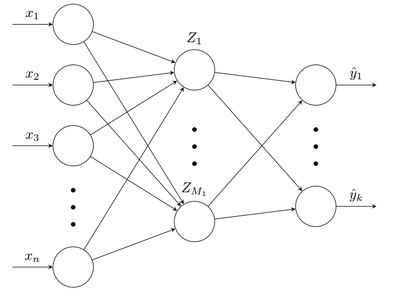
\includegraphics[width=0.5\textwidth]{picture1.png} 
    \caption{Red neuronal}
    \label{fig:miImagen} 
\end{figure}

Para cada neurona de la capa oculta, transformamos todos los valores de las neuronas 
de la capa de entrada de la siguiente manera:
\begin{align*}
    a_j^{(1)} &= \sum_{i=1}^n w_{j,i}^{(1)}x_i+b_{j,}^{(1)}\\
    Z_j^{(1)} &= \sigma(a_j)\:, j = 1, 2, \dots M_1
\end{align*}
con $\sigma$ la función de activación y $w_{j,i}$ los pesos asociados a cada neurona, 
además de un peso de la propia neurona receptora, llamada sesgo $b_{j}$. En caso de 
haber más  capas ocultas repitiriamos este proceso:
\begin{align*}
    Z_j^{(m)} = \sigma\left(\sum_{i = 1}^{M_{(m-1)}}w_{j,i}^{(m)}Z_i^{(m-1)}+b_{j}^m\right)
\end{align*}
En este el caso de la figura~\ref{fig:miImagen}, la salida de la red neuronal será:
\begin{align*}
\hat{y}_k = \sigma\left(\sum_{i=1}^{M_1} w_{k,i}^{(2)}Z_i^{(1)}+b_{k}^{(2)}\right)
\end{align*}
Tras obtener los resultados de la primera evaluación, se actualizan los pesos de la 
red intentando inimizar la siguiente función:
\begin{align*}
   \mathcal{L}(y, \hat{y}_i) = \sum_{i=1}^n \rho(y_i - \hat{y}_i)
\end{align*}
Siendo $y_i$ el valor esperado. Es decir, intentamos modificar los pesos de manera que 
la predicción sea lo más parecida al valor real posible. Modificaremos la función $\rho$ 
en función de cual sea el objetivo de cáculo de la red. \\

En cuanto a las funciones de activación, la más utilizada e implementada en la mayoría 
de métodos es la función ReLu:
\begin{align*}
      \sigma(x) = 
      \begin{cases}
         x & \text{si } x > 0 \\
         0 & \text{si } x \leq 0
      \end{cases} = \max(0, x)
\end{align*}


Para ajustar los pesos, utilizaremos el algoritmo de retropropagación (backpropagation), que 
se basa en el cálculo del gradiente de la función de pérdida con respecto a los pesos.
Calculamos el gradiente de la función de pérdida con respecto a los pesos de la 
capa de salida y luego propagamos este gradiente hacia atrás a través de la red para
ajustar los pesos de las capas ocultas. Los errores en cada capa serán:

\begin{align*}
   \delta^{(L)} &= \nabla_{\hat{y}_i} \rho(y_i - \hat{y}_i)\\
   \delta^{(l)} &= \left( w^{(l+1) \, T} \delta^{(l+1)} \right) \circ \sigma'^{(l)}(a^{(l)}) = \left( w^{(l+1)\, T} \delta^{(l+1)} \right) \circ 1_{a^{(l)} > 0}\quad \text{para } l = L-1, \dots, 1
\end{align*}
con $\circ$ el producto elemento a elemento (Hadamard) y:
\begin{align*}
    \left[\mathbf{1}_{a^{(l)} > 0}\right]_j =
    \begin{cases}
        1 & \text{si } a_j^{(l)} > 0 \\
        0 & \text{si } a_j^{(l)} \leq 0
    \end{cases}
\end{align*}
Utilizando estos errores, actualizaremos lo pesos y los sesgos de la red neuronal teniendo 
en cuenta un valor llamado tasa de aprendizaje $\zeta$, que determina la magnitud de los
ajustes en cada iteración. Suponemos, por tanto, que tenemos $m$ datos disponibles 
$(\mathbf{x_1}, y_1), (\mathbf{x_2}, y_2), \dots, (\mathbf{x_m}, y_m)$, donde $\mathbf{x_i}$ 
son las variables explicativas y $y_i$ la variable dependiente. El algormitmo será:\\

\begin{algorithm}[H]
   \caption{Red neuronal}
   Inicializar aleatoriamente los pesos $w^{(l)}$ y sesgos $b^{(l)}$ para $l = 1, \dots, L$\;
   \For{$\tau = 1$ \KwTo $T$}{
       \For{$i = 1$ \KwTo $m$}{
           \tcp*[l]{Propagación hacia adelante}
           $Z^{(0)} \gets \mathbf{x}_i$\;
           \For{$l = 1$ \KwTo $L-1$}{
               $a^{(l)} \gets w^{(l)} Z^{(l-1)} + b^{(l)}$\;
               $Z^{(l)} \gets \sigma^{(l)}(a^{(l)})$\;
           }
           $a^{(L)} \gets w^{(L)} Z^{(L-1)} + b^{(L)}$\;
           $\hat{y}_i \gets a^{(L)}$\;
   
           \tcp*[l]{Cálculo del error de salida}
           $\delta^{(L)} \gets \nabla_{\hat{y}_i} \rho(y_i - \hat{y}_i)$\;
   
           \tcp*[l]{Retropropagación}
           \For{$l = L$ \KwTo $2$}{
               $w^{(l)} \gets w^{(l)} - \zeta \cdot \delta^{(l)} (Z^{(l-1)})^T$\;
               $b^{(l)} \gets b^{(l)} - \zeta \cdot \delta^{(l)}$\;
               $\delta^{(l-1)} \gets (w^{(l)})^T \delta^{(l)} \circ \mathbf{1}_{a^{(l-1)} > 0}$\;
           }
           $w^{(1)} \gets w^{(1)} - \zeta \cdot \delta^{(1)} (Z^{(0)})^T$\;
           $b^{(1)} \gets b^{(1)} - \zeta \cdot \delta^{(1)}$\;
       }
   }
   \end{algorithm}
\hfil\\
Una de sus principales ventajas es su simplicidad computacional y su capacidad para 
evitar el problema del gradiente desvanecido en regiones positivas, lo que mejora 
significativamente la eficiencia del entrenamiento mediante el método de descenso por 
gradiente. Además, su derivada es muyu simple, lo que  permite una propagación del 
gradiente más estable en comparación con funciones como la sigmoide. \\

Las redes neuronales tienes una gran capacidad de aprendizaje y alta precisión en 
tareas complejas. Estas son las características que hacen que su utilizacióne este muy 
extendida en modelos predictivos.\\

\subsection{Algoritmos de Boosting}
El boosting asume la existencia de algoritmos débiles que, dados ejemplos de 
entrenamiento etiquetados, produce un predictores débiles. Supone que a continuación, 
la combinación de estos predictores débiles producen un predictor fuerte de alta precisión.\\

El objetivo es ir generando estos predictores de forma iterativa. Para que sean diferentes, 
tendremos que modificar el peso o importancia de cada dato dentro de la muestra, 
para que cada clasificador débil se ''especialice'' en unos pocos datos. El peso de cada 
dato se modificará según la predicción hasta ese momento este cerca del valor real o no. \\

Los algoritmos de Boosting se basan en minimizar una función de pérdida de forma 
iterativa, ajustando cada nuevo modelo para corregir los errores de los modelos anteriores.\\

Para ajustar el modelo, debemos entrenarlo, al igual que ocurre con las redes 
neuronales. Por tanto, para la explicación del modelo, tomamos 
$(\mathbf{x_1}, y_1), (\mathbf{x_2}, y_2), \dots, (\mathbf{x_n}, y_n)$, siendo $\mathbf{x_i}$ 
variables explicativas y $y_i$ la variable dependiente. \\

Al igual que anteriormente, el objetivo del algoritmo será minimizar una función de pérdida 
y, una vez obtenido el predictor débil que minimiza este error, lo añadiremos al predictor 
fuerte y modificaremos los pesos de los datos de entrenamiento. Denotaremos la 
función de pérdida de la siguiente manera:
\begin{align*}
   L(y, f(x)) =\sum_{i=1}^n \rho(y_i-f(x_i))
\end{align*}

La función de pérdida $\rho$ será modificada en función del objetivo de cáculo 
del algoritmo de boosting. Para calcular cuantiles, utilizaremos la función de pérdida 
cuantil o \textit{pinball loss} y para calcular expectiles utilizaremos la función de pérdida 
expectil, ambas ya presentadas anteriormente.\\

El algoritmo de boosting es ideal para afrontar el problema ya que $\mathbf{x_i}$ es una 
variable multidimensional y el problema puede tornarse complejo. La eficiencia y precisión 
de los algoritmos de boosting los hacen muy útiles en la estimación de cuantiles y 
expecitles.\\

Vamos a utilizar árboles de regresión como predictores débiles. Un árbol de regresión 
dividirá el conjunto de datos de entrenamiento según los valores de las variables
independientes. En cada nodo, el algoritmo elige la variable y el umbral que minimizan 
la pérdida cuantil o expectil.\\

Para la optimización de los predictores utilizaremos el gradiente descendente, explicado 
anteriormente. En este contexto, aplicamos el gradiente descendente para mejorar la 
función de predicción en cada iteración del algoritmo de boosting.\\

Además, deberemos dar un valor a lo que nuestro predictor final ``aprende'' en cada 
iteración, asignando un valor a lo que llamaremos la tasa de aprendizaje, $\eta$. En 
principio, el valor de la tasa de aprendizaje será un valor pequeño para que el predictor 
vaya aprendiendo poco a poco. Lo haremos de la siguiente manera:


\begin{algorithm}[H]
   \caption{Boosting para cuantiles y expectiles}
   
   Inicializar $f_0(x) \gets 0$ o $f_0(x) \gets \bar{y}$ (la media de los valores $y_i$)\;
   
   \For{$m = 1$ \KwTo $M$}{
       \For{$i = 1$ \KwTo $n$}{
           $u_{i,m} \gets -\rho'_\tau(y_i - f_{m-1}(x_i))$\;
           $u_{i,m} \gets \mathbb{I}(y_i - f_{m-1}(x_i) < 0)(\tau - 1)$\;
       }
   
       \tcp*[l]{Ajustar un predictor débil $g_m(x)$ a los pares $(x_i, u_{i,m})$}
         $\{(x_i, u_{i,m}) \}_{i=1}^n \longrightarrow g_m(x)$\;
       $f_m(x) \gets f_{m-1}(x) + \eta \cdot g_m(x)$\;
   }
   \end{algorithm}
   


\chapter{Aplicaciones de modelos a datos de créditos}
---------------Todo esto ponerlo enla zona de aplicación para explicar los métodos-------------------------
Como ya hemos comentado, el modelo tiene asociado unos parámetros entre los que se encuentran la tasa de aprendizaje y la profundidad
maxima que puede alcanzar un predictor débil (árbol de regresión). Estos parámetros son los que van a determinar la complejidad del modelo y su capacidad de ajuste.\\
Para obtener los parámetros óptimos, utilizaremos una función de medida de la correción del ajuste e iteraremos distintos valores de los parámetros.\\

La función de medida que vamos a utilizar la función de pérdida, llamada "Mean Pinball Loss":
\begin{align*}
   pinball(y, \hat{y}) = \frac{1}{n}\sum_{i=1}^n\rho_{\tau}(y_i-\hat{y}_i)
\end{align*}
\[
   \hat{c}(x) =
   \begin{cases}
      -\sum_{i=0}^{k} b[i] \cdot x[i] - capacidad\cdot(p-k) & \text{si caben en el tren} \\
      +\infty & \text{si no caben en el tren}
   \end{cases}
\]
Para su elección, utilizaremos el método de validación cruzada. Este método consiste en dividir el conjunto de datos en $k$ partes, de las cuales $k-1$ se utilizan para entrenar el modelo y la restante para evaluar su rendimiento. Este proceso se repite $k$ veces, cada vez utilizando una parte diferente como conjunto de prueba. Al final, se promedian los resultados obtenidos en cada iteración para obtener una estimación más robusta del rendimiento del modelo.\\
\clearemptydoublepage
\chapter{Medidas de riesgo}

Incluimos en este capítulo algunos comentarios generales y consejos de escritura 
que no se refieren específicamente a esta plantilla.

\section{VaR}

Como en cualquier documento escrito en {\LaTeX} (en nuestro caso, 
\emph{pdflatex}) podemos incluir figuras. Estas figuras pueden ser imágenes 
contenidas en documentos aparte o compuestas dentro de nuestro documento con 
órdenes de \LaTeX. Se pueden incluir imágenes en diversos formatos 
gráficos, como pdf, jpeg y png, pero no todos; por 
ejemplo, no se pueden incluir imágenes tiff o gif.

Es preferible dejar flotar las figuras. Si se usa el entorno \emph{figure}, 
entonces con
\begin{verbatim}
\begin{figure}[ht]
...
\end{figure}
\end{verbatim}
indicamos que la figura debe insertarse preferiblemente donde se escribe el 
código (la \texttt{h} de \emph{here}) o en la parte superior de la página (la 
\texttt{t} de \emph{top}).

%--------------
\begin{figure}[ht]% h (here) o t (top)
\centering

\includegraphics[width=0.45\textwidth]{ciencias.png}
\qquad

\includegraphics[width=0.45\textwidth]{logoUZ.png}
\caption{dos imágenes en archivos externos.}
\end{figure}
%--------------

El paquete \emph{tikz} permite hacer gráficas de funciones, 
figuras geométricas y diagramas sencillos, y no tan sencillos, como los de las 
figuras~\ref{graf-seno} y~\ref{dosjuntas}.

%--------------
\begin{figure}[ht]% h (here) o t (top)
\centering
% xscale, yscale sirven para escalar en horizontal y vertical
\begin{tikzpicture}[xscale=0.8, yscale=1.2]
% La curva
\draw[very thick, color=blue] plot[domain=-2*pi:3*pi, samples=200] (\x, {sin(2*\x r)});
% Eje horizontal
\draw[thin, gray] (-2*pi-0.3,0) -- (3*pi+0.3,0);
% Eje vertical
\draw[thin, gray] (0,-1) -- (0,1);
\end{tikzpicture}
\caption{gráfica de la función $\sen(2x)$ entre $-2\pi$ y $3\pi$, hecha con \emph{tikz}.}
\label{graf-seno}
\end{figure}
%--------------

%--------------
\begin{figure}[ht]% h (here) o t (top)
\centering
\begin{tikzpicture}[scale=0.8]
% Ejes de coordenadas
\draw (-1,0) -- (5,0);
\draw (0,-1) -- (0,3);

% Puntos en coordenadas polares: (30:4) [observa los dos puntos]
% 30 es el ángulo en grados
% 4 es el módulo
% la orden -latex indica que el segmento termina en una flecha estilo LaTeX
\draw[very thick, red, -latex] (0,0) -- (30:4);

% (30:4 |- 0,0) indica la intersección de dos rectas:
% la recta que parte del punto (30:4) [observa que está en polares]
% en vertical [observa el símbolo |]
% y la recta que parte en horizontal [observa el símbolo -]
% del punto (0,0) [observa que está en cartesianas]
\draw[very thin, gray] (30:4) -- (30:4 |- 0,0);
\draw[very thin, gray] (30:4) -- (30:4 -| 0,0);

% arco de circunferencia terminado en flecha [-latex]
% que empieza en el punto (0:2) [observa que está en polares]
% que tiene ángulo de salida 0,
% ángulo de llegada 30
% y radio 2
\draw[-latex] (0:2) arc (0:30:2);

% Rótulos
% Primero: (a,b) en el punto (30;4),
% pero dejando el punto (30:4) al suroeste (abajo a la izquierda)
\draw (30:4) node[anchor=south west]{$(a,b)$};
% Segundo:
\draw (15:2) node[anchor=west]{$\alpha$};
% Tercero:
\draw (30:4 |- 0,0) node[below]{$(a,0)$};
% Cuarto:
\draw (30:4 -| 0,0) node[left]{$(0,b)$};
\end{tikzpicture}
%--------------
\qquad
%--------------
\begin{tikzpicture}[scale=1.2,
% Estilo de los círculos
circ/.style={circle, inner sep=0pt, minimum size=35pt, thick, draw=blue, fill=blue!10!white},
% Estilo de las flechas
flecha/.style={-latex,shorten >=2pt, shorten <=2pt, color=blue, very thick},
]
% Nodos
\node (4) at (0,0) [circ]{$4$};
\node (5) at (2,1) [circ]{$5$};
\node (6) at (2,-1) [circ]{$6$};

% Flechas
\draw[flecha] (5) to [bend right=15] (6);
\draw[flecha] (6) to [bend right=15] (5);
\end{tikzpicture}
\caption{dos figuras juntas hechas con \emph{tikz}.}
\label{dosjuntas}
\end{figure}
%--------------

\section{CoVar}
\label{etiquetas}

A menudo, los capítulos y secciones, los enunciados (teoremas, proposiciones, 
corolarios\dots) y las figuras llevan una numeración 
automática. Las fórmulas centradas pueden llevar 
también numeración o no llevarla. Es mejor numerar solo las fórmulas a las que se 
hace referencia en el texto. En cualquier caso, nunca se debe numerar \emph{a 
mano}, sino usar las órdenes de {\LaTeX} adecuadas; por ejemplo,
\begin{verbatim}
\begin{equation}
...
\end{equation}
\end{verbatim}
Y tampoco se debe hacer referencia a las fórmulas y enunciados escribiendo a mano 
la numeración, sino etiquetando la fórmula o enunciado con \verb"\label"  y 
refiriéndonos a ellos con \verb"\eqref" (para fórmulas) y \verb"\ref" (para 
enunciados).

De la misma manera, para hacer referencia a una entrada de la bibliografía 
debemos usar la orden \verb"\cite", nunca escribir a mano la clave.

\section{Déficit esperado (Expected Shotfall)}

Al escribir un trabajo hay algunas reglas de estilo a las que conviene atenerse. 
Es fácil encontrar textos, más o menos exhaustivos, que recogen estas reglas. 
Aunque en ocasiones no queramos seguirlas hasta el último detalle, es útil 
releerlas de vez en cuando.

En la bibliografía hemos seleccionado algunas referencias con indicaciones sobre 
{\LaTeX}, tipografía y lingüística (\cite{ALV,B,RAE}).

Es singularmente interesante la página \emph{texnia}
(\url{http://www.texnia.com/}) de Javier Bezos, una autoridad en \LaTeX y tipografía. Ahí está 
disponible~\cite{B}, entre mucha más información.

La guía~\cite{ALV} está escrita para los alumnos de la Universidad de La Rioja que redacten su 
trabajo de fin de grado en \LaTeX. De ella hemos tomado buena parte de estas notas. Uno de sus 
autores, Juan Luis Varona, es otro gran experto en {\LaTeX}, edición y tipografía.

%De~\cite{V}, escrita para La Gaceta de la Real Sociedad Matemática Española, 
%recomendamos también las referencias que contiene. Su autor, Juan Luis Varona, es 
%otro gran experto en {\TeX}, edición y tipografía.

%En~\cite{M} se puede ver una lista bastante amplia de normas concretas para 
%trabajos escritos en {\LaTeX}.

Desde luego, para cualquier duda lingüística en castellano es indispensable la 
página de la Real Academia Española~\cite{RAE}, donde encontraremos su 
diccionario de la lengua española y su diccionario panhispánico de dudas.

Recogemos aquí algunos primeros consejos:
\begin{enumerate} 
\item Redacta correctamente. Aunque se trate de un texto matemático, debe estar 
bien escrito y sin faltas de ortografía o gramaticales.

\item Escribe un buen código {\LaTeX}. Un código claro, bien estructurado, es más 
fácil de repasar. Lo que parece sencillo de entender en el momento en que lo 
escribes, puede resultar oscuro si lo tienes que revisar al cabo de un tiempo. 
Pon comentarios (líneas que empiezan por~\%) para explicar las partes más 
complicadas.

\item Corrige todos los errores de {\TeX} que ocurran al componer el texto. No te 
conformes nunca con pulsar \emph{Enter} hasta que salga el pdf. Intenta obtener 
al final una composición limpia, sin errores ni 
advertencias. En particular, sin avisos de \emph{overfull}.

\item No incluyas una inmensa lista de paquetes o definiciones 
que no vas a usar, a menudo copiados y pegados de otros sitios.

\item Usa los entornos del tipo teorema, definición, observación{\dots} (es 
decir, con \verb"\begin{teorema}", \dots, \verb"\end{teorema}"), en lugar de 
formatear a mano los enunciados.

\item No cites nunca a mano las fórmulas y enunciados; no pongas numeración a 
fórmulas que no cites. Sobre esto hemos comentado algo en la 
sección~\ref{etiquetas}.

\item Evita, si es posible, las órdenes \verb"\bigskip", \verb"\medskip", 
\verb"\smallskip", \verb"\hskip", \verb"\vskip" y similares, y no uses \verb"\ ", 
\verb"\," y análogas sin una buena razón. Es decir, como regla general es mejor 
dejar que {\LaTeX} establezca el espaciado vertical y horizontal por sí mismo.

\item Haz un uso moderado de \verb"\emph", \verb"\textbf" y similares: una 
palabra en cursiva o negrita llama la atención, pero 
una página llena de cursivas, negritas, texto entre comillas, recuadros o incluso 
distintos colores es simplemente más difícil de leer. Decide con qué criterio vas 
a usar cada uno de estos recursos tipográficos.

\item Consulta un buen manual, como~\cite{CLMPS} y~\cite{MGBCR}, antes de escribir una expresión matemática nueva. Es probable que allí 
encuentres una solución más sencilla que la que vayas a desarrollar por tu 
cuenta. La mayoría de los paquetes tienen también su manual, que tendrás en tu 
distribución de {\LaTeX}.

\item Hay una gran variedad de órdenes para escribir fórmulas que no caben en una 
línea. Consulta la guía de 
usuario del paquete \emph{amsmath}.

\item Establece un estilo para la bibliografía y sujétate a 
él. Esto también lo hemos comentado antes, en la sección~\ref{bibliografia}. Ten 
en cuenta, para decidir el estilo, que las entradas de la bilbiografía pueden ser 
de varios tipos: libros enteros, artículos de revistas, páginas web{\dots} Puedes 
tomar el estilo de alguna revista, por ejemplo.

\item No abrevies los nombres de las revistas de cualquier manera: hay formas 
normalizadas de hacerlo. Puedes consultar las abreviaturas de revistas 
matemáticas en~\cite{A}, de la American 
Mathematical Society (AMS). También puedes consultar MathSciNet (por 
ejemplo,~\cite{A2}), así mismo de la AMS y suscrita por la Universidad de 
Zaragoza. Si no encuentras la revista que quieres, puedes buscar en~\cite{I} las 
abreviaturas de palabras en títulos de revistas, en diferentes idiomas, según la 
norma ISO.
\end{enumerate}
%--- FIN DEL CAPÍTULO 2

%--- CAPÍTULO 3 DEL TFG
\section{Modelos de riesgo}

El contenido de la sección~\ref{Gamma-producto} está tomado, sin apenas cambios, 
de~\cite[pág.~518 y sig.]{BC}. Y el de la sección~\ref{Gamma-integral}, 
de~\cite[pág.~185--187]{C} y~\cite[pág.~206 y sig.]{W}. De las muchas 
demostraciones de la fórmula de Stirling, la que presentamos en la 
sección~\ref{fStirling} está tomada esencialmente de~\cite{P}.

Para la primera sección es necesario tener conocimientos de análisis complejo. 
Damos por conocida la factorización
\begin{equation}
\label{factor-seno}
   \sen \pi z = \pi z \prod_{n=1}^\infty \left(1 - \frac{z^2}{n^2} \right),
   \qquad z \in \C,
\end{equation}
cuya demostración puede verse, por ejemplo, en~\cite[pág.~518]{BC} o 
en~\cite[pág.~211--212]{W}.

Enunciamos aquí el teorema de factorización que 
usamos en la sección~\ref{Gamma-producto} (en realidad, el teorema de 
factorización de Weierstrass es más bien un recíproco de este resultado):
\begin{defin}
Escribimos $E_0(w) = 1 - w$ y para cada $p \in \N$,
\[
   E_p(w) 
   = (1-w) \exp\left(w + \frac{w^2}{2} + \frac{w^3}{3} + \dots + \frac{w^p}{p}\right).
\]
Estas funciones enteras se llaman \emph{factores elementales} y su único cero 
es~$1$, simple.
\end{defin}

\begin{teorema}
Sea $\{z_n\}_{n=1}^\infty \subseteq \C$ con $z_n \not= 0$ para todo $n$ y $z_n 
\to \infty$ (pueden estar repetidos). Si $\{p_n\}_{n=1}^\infty \subseteq \N \cup 
\{0\}$ y para cada $r > 0$ la serie
\[
   \sum_{n=1}^\infty \left(\frac{r}{|z_n|}\right)^{1+p_n}
\]
converge, entonces:
\begin{enumerate}
\item[a)] $f(z) = \prod\limits_{n=1}^\infty E_{p_n}(\frac{z}{z_n})$ define una 
función holomorfa en $\C$;
\item[b)] los ceros de $f$ son los $z_n$ y su multiplicidad es el número de veces 
que aparecen repetidos en la sucesión.
\end{enumerate}
\end{teorema}

%------
\subsection{Modelos clásicos}
\label{Gamma-producto}

La función entera más sencilla que se anula, con ceros 
simples, en los enteros negativos es
\begin{equation}
\label{defF}
   F(z) = \prod_{n=1}^\infty \left(1 + \frac{z}{n}\right) e^{-z/n}.
\end{equation}
\subsection{Modelo GARCH}
En efecto, basta aplicar el teorema de 
factorización con $z_n = -n$ para cada $n \in \N$ 
y con $p_n = 1$; claramente, para cada $r > 0$ la serie
\[
   \sum_{n=1}^\infty \left( \frac{r}{|z_n|} \right)^{1+p_n}
   = \sum_{n=1}^\infty \frac{r^2}{n^2}
\]
converge, y entonces el producto infinito
\[
   \prod_{n=1}^\infty E_{p_n}\left(\frac{z}{z_n}\right)
   = \prod_{n=1}^\infty \left(1 - \frac{z}{z_n}\right) e^{z/z_n}
   = \prod_{n=1}^\infty \left(1 + \frac{z}{n}\right) e^{-z/n}
\]
converge uniformemente sobre 
compactos de $\C$ y define una 
función entera cuyos ceros son los enteros negativos, todos ellos simples.

De la factorización~\eqref{factor-seno}
se deduce que
\[
   \sen \pi z = \pi z F(z) F(-z).
\]
Las funciones $F(z-1)$ y $z F(z)$ son ambas enteras y con los mismos ceros: $0, 
-1, -2 \dots$, todos ellos simples. Por lo tanto, su cociente tiene logaritmo 
holomorfo: es una función entera que no se anula en ningún punto. Es decir:
\begin{equation}
\label{Fzz-1}
   F(z-1) = z F(z) e^{g(z)}
\end{equation}
para alguna función entera $g$. Si sustituimos $F$ por su definición, tenemos
\[
   \prod_{n=1}^\infty \left(1 + \frac{z-1}{n}\right) e^{-\frac{z-1}{n}}
   = z e^{g(z)} \prod_{n=1}^\infty \left(1 + \frac{z}{n}\right) e^{-z/n}.
\]
En esta expresión tomamos \emph{derivadas logarítmicas}:
\[
   \sum_{n=1}^\infty \left( \frac{1/n}{1 + \frac{z-1}{n}} - \frac{1}{n} \right)
   = \frac{1}{z} + g'(z)
   + \sum_{n=1}^\infty \left( \frac{1/n}{1 + \frac{z}{n}} - \frac{1}{n} \right).
\]
No insistiremos en esto, pero todos los productos infinitos, las series y los 
límites que hemos manejado y los que vengan a continuación convergen porque 
converge el producto infinito~\eqref{defF} y porque se puede derivar 
logarítmicamente.

De la fórmula anterior obtenemos $g'(z)$, pasando a sumas parciales para no 
manejar series que no converjan:
\begin{align*}
   \frac{1}{z} + g'(z)
   &= \sum_{n=1}^\infty
   \left( \frac{1/n}{1 + \frac{z-1}{n}} - \frac{1/n}{1 + \frac{z}{n}} \right)
   = \lim_N \sum_{n=1}^N
   \left( \frac{1}{n + z-1} - \frac{1}{n + z} \right)
   \\
   &= \lim_N \left( \frac{1}{z} - \frac{1}{N + z} \right)
   = \frac{1}{z}.
\end{align*}
Por consiguiente, $g'(z) = 0$ para todo $z \in \C$, es decir, $g$ es una 
constante. ¿Qué constante? La llamamos~$\gamma$ y para hallarla basta imponer que 
cumpla la fórmula~\eqref{Fzz-1} sustituyendo, por ejemplo, $z=1$:
\[
   1 = F(0) = F(1) e^\gamma 
   = e^\gamma \prod_{n=1}^\infty \left(1 + \frac{1}{n}\right) e^{-1/n},
\]
es decir,
\[
   e^{-\gamma} = \prod_{n=1}^\infty \left(1 + \frac{1}{n}\right) e^{-1/n}.
\]
Naturalmente, no hay un único valor porque el logaritmo complejo no es único, 
pero el producto infinito de la derecha es un número real positivo y entonces 
podemos elegir el único $\gamma \in \R$ que cumple esa relación. Es decir:
\[
   \gamma = - \log \prod_{n=1}^\infty \left(1 + \frac{1}{n}\right) e^{-1/n}
   = - \log \lim_N \prod_{n=1}^N \frac{n+1}{n} e^{-1/n}
   = - \log \lim_N (N+1) e^{-1 - \frac{1}{2} - \ldots - \frac{1}{N}}.
\]
O, equivalentemente:
\[
   \gamma = \lim_N \left(
   1 + \frac{1}{2} + \dots + \frac{1}{N} - \log(N+1)
   \right).
\]
Esta constante se llama \emph{constante de Euler}. 
Observemos que como $\log (N+1) = \log N + \log (1 + \frac{1}{N})$, también 
podemos escribir
\begin{equation}
\label{gamma}
   \gamma = \lim_N \left(
   1 + \frac{1}{2} + \dots + \frac{1}{N} - \log N
   \right).
\end{equation}
Volviendo a la fórmula~\eqref{Fzz-1}, pero ya con $g(z) = \gamma$, tenemos
\[
   F(z-1) = z F(z) e^\gamma
\]
y por lo tanto
\[
   e^{\gamma(z-1)} F(z-1) = z e^{\gamma z} F(z).
\]
La función $\Gamma(z) = \frac{1}{z e^{\gamma z} F(z)}$, cuyos polos son $0, -1, 
-2 \dots$, todos ellos simples, cumple
\begin{gather*}
   \Gamma(z+1) = \frac{1}{e^{\gamma z} F(z)} = z \Gamma(z),
   \\
   \Gamma(1) = \frac{1}{e^\gamma F(1)} = 1.
\end{gather*}
En particular, de aquí se deduce por inducción que $\Gamma(n) = (n-1)!$ para todo 
$n \in \N$. También se cumple que
\[
   \sen \pi z = \pi z F(z) F(-z)
   = \pi z \frac{1}{z e^{\gamma z} \Gamma(z)} 
   \cdot \frac{1}{-z e^{-\gamma z} \Gamma(-z)}
   = \frac{\pi}{\Gamma(z) (-z) \Gamma(-z)}
   = \frac{\pi}{\Gamma(z) \Gamma(1-z)},
\]
es decir,
\[
   \Gamma(z) \Gamma(1-z) = \frac{\pi}{\sen \pi z},
   \quad z \notin \Z.
\]
Si hacemos $z = 1/2$, obtenemos $\Gamma(1/2)^2 = \pi$. Como
\[
   \Gamma(\tfrac{1}{2}) 
   = \frac{1}{\frac{1}{2} e^{\frac{1}{2}\gamma} F(\frac{1}{2})}
   = \frac{1}{\frac{1}{2} e^{\frac{1}{2}\gamma} 
   \prod_{n=1}^\infty (1 + \frac{1}{2n}) e^{-\frac{1}{2n}}}
   > 0,
\]
se deduce que
\[
   \Gamma(\tfrac{1}{2}) = \sqrt{\pi}.
\]
Por otra parte, de la definición de $\Gamma(z)$ se sigue que
\[
   \Gamma(z) = \frac{e^{-\gamma z}}{z} 
   \prod_{n=1}^\infty \left(1 + \frac{z}{n}\right)^{-1} e^{z/n},
   \quad z \not= 0, -1, -2 \dots
\]
Por lo tanto,
\begin{align*}
   \Gamma(z) &= \frac{e^{-\gamma z}}{z} 
   \lim_N \prod_{n=1}^N \left(1 + \frac{z}{n}\right)^{-1} e^{z/n}
   = \lim_N \frac{e^{-\gamma z} N! e^{z(1+\frac{1}{2}+\dots+\frac{1}{N})}}
   {z (z+1) \dots (z+N)}
   \\
   &= \lim_N \frac{e^{z \log N} N!}{z (z+1) \dots (z+N)}
   e^{z(-\gamma+1+\frac{1}{2}+\dots+\frac{1}{N}-\log N)}.
\end{align*}
Teniendo en cuenta~\eqref{gamma}, queda
\[
   \Gamma(z) = \lim_N \frac{N^z N!}{z (z+1) \dots (z+N)},
   \quad z \not= 0, -1, -2 \dots
\]
La función $\Gamma$ se llama \emph{función $\Gamma$ de Euler}.

%------
\subsection{Modelos de aprendizaje automático}
\label{Gamma-integral}

La definición más clásica de la función $\Gamma$ es como una integral:
\[
   \Gamma(z) = \int_0^\infty t^{z-1} e^{-t} \, dt,
   \quad \Re z > 0.
\]
Vamos a ver que esta definición coincide con la anterior. De momento, definamos
\[
   G(z) = \int_0^\infty t^{z-1} e^{-t} \, dt.
\]

\subsection{Modelo XGBoost}
Como $|t^{z-1} e^{-t}| = t^{\Re(z)-1} e^{-t}$, se deduce que la función $G$ está 
bien definida si $\Re z > 0$. En realidad, es fácil comprobar que es una función 
holomorfa en el abierto $\{z \in \C; \Re z > 0\}$. 
Algunas propiedades sencillas de esta función son:
\begin{enumerate}
\item[a)] $G(z+1) = z G(z)$ (se comprueba integrando por partes).
\item[b)] $G(1) = 1$ (es una integral inmediata).
\item[c)] Para cada $n \in \N$, $G(n) = (n-1)!$ (se prueba por inducción, a 
partir de las dos propiedades anteriores).
\end{enumerate}
Sean ahora $x, y > 0$ (números reales positivos), $0 < \lambda < 1$. Entonces,
\[
   G(\lambda x + (1-\lambda)y)
   = \int_0^\infty t^{\lambda x + (1-\lambda)y - 1} e^{-t} \, dt
   = \int_0^\infty t^{\lambda (x-1)} e^{-\lambda t}
   t^{(1-\lambda)(y-1)} e^{-(1-\lambda)t} \, dt.
\]
Aplicamos ahora la desigualdad de Hölder a las 
funciones $t^{\lambda (x-1)} e^{-\lambda t}$, $t^{(1-\lambda)(y-1)} e^{-(1-
\lambda)t}$, con exponentes $p = 1/\lambda$, $q = 1/(1-\lambda)$. Resulta:
\begin{align*}
   G(\lambda x + (1-\lambda)y)
   &\leq \left(\int_0^\infty t^{\lambda p (x-1)} e^{-\lambda p t}
   \, dt \right)^{1/p}
   \left(\int_0^\infty t^{(1-\lambda) q (y-1)} e^{-(1-\lambda) qt}
   \, dt \right)^{1/q}
   \\
   &= \left(\int_0^\infty t^{x-1} e^{-t} \, dt \right)^\lambda
   \left(\int_0^\infty t^{y-1} e^{-t} \, dt \right)^{1-\lambda}.
\end{align*}
Es decir:
\[
   G(\lambda x + (1-\lambda)y) \leq G(x)^\lambda G(y)^{1-\lambda},
   \quad x > 0, \ y > 0, \ 0 \leq \lambda \leq 1
\]
(los casos $\lambda = 0$, $\lambda = 1$ son triviales). Las funciones que cumplen 
esta propiedad se llaman 
\emph{logarítmicamente convexas}.

La demostración que vamos a ver de que $G$ es la función $\Gamma$ se aplica a 
cualquier función $G : (0,\infty) \to (0,\infty)$ que cumpla las propiedades 
\emph{a)}, \emph{b)}, \emph{c)} y la convexidad logarítmica; es el teorema de 
Bohr-Mollerup. En nuestro caso, como $G$ y $
\Gamma$ son holomorfas, si coinciden en $(0,\infty)$ coinciden en todo el abierto 
conexo $\{z \in \C; \Re z > 0\}$, por el principio de prolongación 
analítica.

Comencemos por un $x \in (0,1]$. Sea $n \in \N$. Entonces,
\[
   n + 1 + x = (1-x) (n+1) + x (n+2),
\]
luego, por la convexidad logarítmica (por 
eso hace falta $0 < x \leq 1$),
\begin{align*}
   G(n+1+x) &\leq G(n+1)^{1-x} G(n+2)^x
   = G(n+1)^{1-x} \left[ (n+1) G(n+1) \right]^x
   \\
   &= (n+1)^x G(n+1)
   = (n+1)^x n!
\end{align*}
De la misma manera,
\[
   n + 1 = x (n+x) + (1-x)(n+1+x),
\]
luego
\begin{align*}
   n! &= G(n+1) \leq G(n+x)^x G(n+1+x)^{1-x}
   \\
   &= \left[\frac{G(n+1+x)}{n+x} \right]^x G(n+1+x)^{1-x}
   = \frac{G(n+1+x)}{(n+x)^x}.
\end{align*}
Juntando las dos desigualdades tenemos
\[
   (n+x)^x n! \leq G(n+1+x) \leq (n+1)^x n!,
\]
es decir:
\[
   \left( 1 + \frac{x}{n} \right)^x 
   \leq \frac{G(n+1+x)}{n! \, n^x}
   \leq \left( 1 + \frac{1}{n} \right)^x.
\]
Si hacemos $n \to \infty$, deducimos que
\[
   1 = \lim_n \frac{G(n+1+x)}{n! \, n^x}
   = \lim_n \frac{x (x+1) (x+2) \dots (x+n) G(x)}{n! \, n^x},
\]
donde en el último paso se usa la propiedad \emph{a)}. Por lo tanto,
\[
   G(x) = \lim_n \frac{n! \, n^x}{x (x+1) (x+2) \dots (x+n)} = \Gamma(x).
\]
Ya tenemos que $G(x) = \Gamma(x)$ si $x \in (0,1]$. Para $x > 1$ tendremos $x \in 
(m,m+1]$ para algún $m \in \N$ y entonces
\[
   G(x) = (x-1) (x-2) \dots (x-m) G(x-m)
   = (x-1) (x-2) \dots (x-m) \Gamma(x-m)
   = \Gamma(x).
\]

%------

Partimos de la definición de la función $\Gamma$ como una integral, pero nos 
limitamos a valores reales:
\[
   \Gamma(x) = \int_0^\infty t^{x-1} e^{-t} \, dt,
   \quad x > 0.
\]
Haciendo el cambio de variable $u = \sqrt{t}$, resulta
\[
   \Gamma(x) = \int_0^\infty 2 u^{2x-1} e^{-u^2} \, du.
\]
Por lo tanto,
\[
   \frac{\Gamma(x)}{x^{x-\frac{1}{2}} e^{-x}}
   = \int_0^\infty 2 \left(\frac{u}{\sqrt{x}}\right)^{2x-1} e^{x-u^2} \, du
   = \int_{-\sqrt{x}}^\infty 2 \left(1 + \frac{v}{\sqrt{x}}\right)^{2x-1}
   e^{-2v\sqrt{x}} e^{-v^2} \, dv,
\]
donde para llegar a la segunda integral hacemos el cambio $u = \sqrt{x} + v$ (así 
que $x - u^2 = -2v \sqrt{x} - v^2$). Es decir,
\begin{equation}
\label{dominada}
   \frac{\Gamma(x)}{x^{x-\frac{1}{2}} e^{-x}}
   = \int_{-\infty}^\infty \chi_{[-\sqrt{x},+\infty)}(x)
   2 \left(1 + \frac{v}{\sqrt{x}}\right)^{2x-1}
   e^{-2v\sqrt{x}} e^{-v^2} \, dv.
\end{equation}
Queremos hacer $x \to +\infty$ usando el teorema de la convergencia 
dominada, para lo cual debemos 
encontrar una acotación y hallar un límite del integrando. En todo lo que sigue 
podemos suponer que $2x - 1 >0$. Empezamos con la acotación: usando la 
desigualdad
\[
   1 + t \leq e^t, \qquad \forall t \in \R,
\]
que se demuestra muy fácilmente, deducimos que
\[
   \left(1 + \frac{v}{\sqrt{x}}\right)^{2x-1}
   \leq e^{2 v \sqrt{x} - \frac{v}{\sqrt{x}}}
\]
y, por lo tanto,
\[
   0 \leq 2 \left(1 + \frac{v}{\sqrt{x}}\right)^{2x-1} e^{-2v\sqrt{x}}
   \leq 2 e^{-v/\sqrt{x}}
   \leq 2 e,
   \quad \text{si } v \in [-\sqrt{x},+\infty).
\]
Así que
\[
   0 \leq \chi_{[-\sqrt{x},+\infty)}(x)
   2 \left(1 + \frac{v}{\sqrt{x}}\right)^{2x-1}
   e^{-2v\sqrt{x}} e^{-v^2}
   \leq 2 e e^{-v^2}.
\]
Ya tenemos la acotación. Ahora, fijado $v \in [-\sqrt{x},+\infty)$,
\[
   2 \left(1 + \frac{v}{\sqrt{x}}\right)^{2x-1}
   e^{-2v\sqrt{x}}
   = 2 e^{(2x-1) \log(1+\frac{v}{\sqrt{x}}) - 2 v \sqrt{x}},
\]
y
\begin{align*}
   \lim_{x \to +\infty} \left( (2x-1) \log(1+\frac{v}{\sqrt{x}}) - 2 v \sqrt{x}
   \right)
   &=\lim_{x \to +\infty} \left( 2x \log(1+\frac{v}{\sqrt{x}}) - 2 v \sqrt{x}
   \right)
   \\
   &= \lim_{x \to +\infty} 2v^2 
   \frac{\log(1+\frac{v}{\sqrt{x}}) - \frac{v}{\sqrt{x}}}{\frac{v^2}{x}}
   \\
   &= \lim_{y \to 0^+} 2v^2 \frac{\log(1+y) - y}{y^2} = - v^2
\end{align*}
(por el desarrollo de Young de $\log(1+y)$ o por la 
regla de L'H\^opital). Es decir, para todo $v \in \R
$,
\[
   \lim_{x \to +\infty} \chi_{[-\sqrt{x},+\infty)}(x)
   2 \left(1 + \frac{v}{\sqrt{x}}\right)^{2x-1}
   e^{-2v\sqrt{x}} e^{-v^2}
   = 2 e^{-2 v^2}.
\]
Llevando todo a~\eqref{dominada}, obtenemos que
\[
   \lim_{x \to +\infty} \frac{\Gamma(x)}{x^{x-\frac{1}{2}} e^{-x}}
   = \int_{-\infty}^{+\infty} 2 e^{-2v^2} \, dv.
\]
Esta integral se calcula de varias maneras. Por ejemplo, usando coordenadas 
polares,
\begin{align*}
   \left( \int_{-\infty}^{+\infty} 2 e^{-2v^2} \, dv \right)^2
   &= \iint_{\R^2} 4 e^{-2 (u^2+v^2)} \, du\, dv
   = \int_{(0.+\infty)} \int_{-\pi}^\pi 4 e^{-2 r^2} r \, d\varphi \, dr
   \\
   &= \int_{(0.+\infty)} 8 \pi r e^{-2 r^2} \, dr
   = \left[ - 2\pi e^{-2 r^2} \right]_{r=0}^{r\to+\infty}
   = 2\pi,
\end{align*}
de donde
\[
   \int_{-\infty}^{+\infty} 2 e^{-2v^2} \, dv = \sqrt{2\pi}.
\]
Así que finalmente obtenemos:
\[
   \lim_{x \to +\infty} \frac{\Gamma(x)}{x^{x-\frac{1}{2}} e^{-x}}
   = \sqrt{2\pi},
\]
que es la fórmula de Stirling. Otra manera equivalente de escribirla, más 
habitual, es esta:
\[
   \lim_{x \to +\infty} \frac{\Gamma(x+1)}{x^x e^{-x} \sqrt{2\pi x}}
   = \lim_{x \to +\infty}
   \frac{x \Gamma(x)}{x^{x+\frac{1}{2}} e^{-x} \sqrt{2\pi}}
   = \lim_{x \to +\infty} \frac{\Gamma(x)}{x^{x-\frac{1}{2}} e^{-x} \sqrt{2\pi}}
   = 1.
\]
%--- FIN DEL CAPÍTULO 3

\clearemptydoublepage
\chapter{Aplicación de QR y XGBoost a ...}
\clearemptydoublepage
\chapter{Análisis de resultados}
\clearemptydoublepage
\chapter{Conclusión}
%-------------
\backmatter                      % Parte final del texto



%------ Bibliografía
% Para meter cosas en el "toc" a mano, ver
% \S 2.3.1 del LaTeX Companion (ejemplo de la p. 47) (Juan Luis)
\phantomsection % Si no, el enlace en el índice apunta a la página anterior
\addcontentsline{toc}{chapter}{\bibname} % Para que salga en el índice general
% Para ponerlo a mano en la cabecera, pues no es \chapter:
\chaptermark{\bibname}
% Cuando no hay secciones para las cabeceras impares, se suele hacer esto:
\sectionmarkwithoutsections{\bibname}

%--- BIBLIOGRAFÍA DEL TFG
\begin{thebibliography}{99}

\bibitem{A}
\textsc{American Mathematical Society},
\textit{Abbreviations of names of serials},
\url{http://www.ams.org/msnhtml/serials.pdf}.

\bibitem{A2}
\textsc{American Mathematical Society},
\textit{MathSciNet} (servidor de Estrasburgo),
\url{http://ams.u-strasbg.fr/mathscinet/}.

\bibitem{ALV}
\textsc{A. Arenas, E. Labarga y J. L. Varona},
\textit{Una breve guía para redactar un trabajo de fin de grado
con contenido matemático utilizando LaTeX},
\url{https://www.unirioja.es/facultades_escuelas/fct/TFG/guia-TFG-matematicas.pdf},
disponible en
\url{https://www.unirioja.es/facultades_escuelas/fct/TFG/guias_manuales.shtml}.

\bibitem{B}
\textsc{J.~Bezos},
\textit{Ortotipografía y notaciones matemáticas},
\url{http://www.texnia.com/archive/ortomatem.pdf},
disponible en
\url{http://www.texnia.com/}.

\bibitem{BC}
\textsc{J. Bruna y J. Cufí},
\textit{An\`alisi complexa},
Colección Manuals, Universitat Aut\`onoma de Barcelona, Bellaterra, 2008.

\bibitem{CLMPS}
\textsc{B. Cascales, P. Lucas, J. M. Mira, A. Pallarés y S. Sánchez-Pedreño}, 
\textit{LaTeX, una imprenta en tus manos}, 
Aula Documental de Investigaci\'on, Madrid, 2000.

\bibitem{C}
\textsc{B. Cuartero},
\textit{Fundamentos de análisis matemático},
Colección Textos Docentes, Prensas Universitarias de Zaragoza, 2009.

\bibitem{FC}
\textsc{Facultad de Ciencias de la Universidad de Zaragoza},
\textit{Directrices propias para la elaboración del trabajo fin de grado en 
Matemáticas}, 
disponible en
\url{https://ciencias.unizar.es/trabajo-fin-de-grado-en-matematicas}.

\bibitem{I}
\textsc{International Standard Serial Number},
\textit{International identifier for serials},
\url{http://www.issn.org/services/online-services/access-to-the-ltwa/}.

%\bibitem{M}
%\textsc{P. Millien},
%\textit{Conseils pour bien taper un document avec {\LaTeX}},
%\url{http://www.math.ens.fr/~millien/tdlatex/conseils_latex.pdf},
%disponible en
%\url{http://www.math.ens.fr/~millien/}.

\bibitem{MGBCR}
\textsc{F. Mittelbach, M. Goossens, J. Braams, D. Carlisle y C. Rowley}, 
\textit{The \LaTeX\ Companion}, 
2.\textsuperscript{a} ed., 
Addison-Wesley, 2004.

\bibitem{P}
\textsc{J. M. Patin},
A very short proof of Stirling's formula,
\textit{Amer. Math. Monthly}
\textbf{96} (1) (1989), 41--42.

\bibitem{RAE}
\textsc{Real Academia Española},
\url{http://www.rae.es/}.

%\bibitem{V}
%\textsc{J. L. Varona},
%\textit{Un ejemplo de cómo escribir un artículo que se publicará en La Gaceta de 
%la RSME},
%\url{http://gaceta.rsme.es/estiloGaceta/articulo-suelto.zip},
%disponible en
%\textit{Información para autores},
%\url{http://gaceta.rsme.es/informacion.php}.

\bibitem{W}
\textsc{R. Webster},
\textit{Convexity},
Oxford University Press, Oxford, 1994.

\end{thebibliography}
%--- FIN DE LA BIBLIOGRAFÍA

%\clearemptydoublepage

\end{document}
